In 2017 the German government passed the law for improvement of online access to administrative services (Online Zugangs Gesetz: OZG) which requires federal republic and member states to execute the following regulations until 2022 \cite{BMI:OZG_Wortlaut}:
\begin{enumerate}
    \item \textbf{Digital availability of administrative services} \\
    An administrative service is the electronic processing of administrative procedures which are available from outside the governmental institution.  As it is not clear which administrative services exactly are meant by the definition of the OZG, the BMI created a catalogue \cite{BMI:Verwaltungsleistungen}. The OZG requires these services to be digitally available. As a guideline to what is considered sufficient availability, the BMI defined a maturity model \cite{BMI:Digitale_Services}.
    \item \textbf{Digital access to administrative services through administration portals of a portal network} \\
    Federal republic, each member state and each commune must provide an administration portal. Portals of communes must be linked to the portal of the corresponding member state. Portals of federal republic and member states must be connected through a portal network. \cite{BMI:Portalverbund} Each portal must provide a "seek and find" feature, which enables users to find all administrative services provided by any administration portal \cite{Cotar:Drucksache_19/19089}. 
    \item \textbf{Interoperable user profiles for accessing administrative services} \\
    Federal republic and member states must provide user profiles which can be used to identify the corresponding person while requesting access to administrative services, to save personal information according to the once-only principle, to receive and send messages via a digital mailbox and to pay for services \cite{Cotar:Drucksache_19/19089}. The user profiles must be interoperable for every administration portal of the portal network.
\end{enumerate}

Execution of the OZG can be separated into two projects:

\paragraph{Digitalization}
Digitalization of administrative services focuses on accessibility towards users but not modernization of its internal execution by administrative institutions. The goal of digitalization in this case is, to make administrative services available towards a user in a digitized way:

A digitized administrative service can be accessed by a user through a website. The website is hosted either by the federal republic or a member state and is called "Administration Portal". Access is usually provided through an application form. The administrative service can be managed through a user profile which is provided by the federal republic or the member state. Management of an administrative service usually includes starting the service by sending in a form, communicating with responsible institutions through the inbox of the profile and receiving a result. The user profile can also enable users to upload documents to a data wallet and to save personal information for automatically filling in forms.

Digitalization of an administrative service is the modification of the underlying processes to incorporate the usage of the described features of the user profile and administration portal. In total, the BMI lists 575 relevant services, some of them provided by the federal republic, some by the member states and yet other by the communes \cite{BMI:Onlinezugangsgesetz}.

\paragraph{Networking}
The networking focuses on connecting governmental systems to make all digitized administrative services available for every user. This includes most importantly the connection of administration portals to a portal network through an online gateway and the interoperability of user profiles.

In order to save investments a method called "one for all" is used when hosting administrative services. One member state or the federal republic provide access to a service on their administration portal and distribute the requests to the responsible institutions "under the hood". As administration portals are connected through an "online gateway", each portal contains a search feature, which enables users to find all administrative services through any portal. Interoperable user profiles enable usage of each profile for management of administrative services on all portals.

\subsection{Basic Use Case}
The BMI lists a total of almost 600 administrative services, each being described by a different process \cite{BMI:Informatiosplattform}. Each process consists of multiple sub-processes. When comparing the processes, one can see, that some sub-processes occur very often and in similar arrangements. Those arrangements can be called the basic use case of OZG services.

The basic use case describes the submission of an application for an administrative service and consists of the following arrangement of sub-processes \cite{NRW:Umsetzung}:

\paragraph{1. Create User Profile}
The user creates a user profile on the administration portal of a member state by entering personal information and a authentication method like username and password or the German digital identity card.

\paragraph{2. Login to User Profile}
Independent of the member state the user created the interoperable user profile for, he can use it in the current administration portal. The user has to finish authentication steps, which can consist for example of a username and password. Depending on the authentication method, a trust level of the current session is determined. With approval from the user, personal information from his profile is provided towards the form-server.

\paragraph{3. Selection of Administrative Service}
The user visits any administration portal of the portal network and types a search term in the corresponding search field. The user is then presented with a list of search results consisting of administrative services. If the user selects a search result, he is forwarded to the correct page inside the domain of the administration portal which hosts the selected service. This page provides information about the administration service along with instructions on how to access the form for application. The interactive form, usually provided by a form-server, can be for example included in the page through a web-component.

\paragraph{4. Filling in Application}
Personal information from the user profile is used by the form-server to fill as many fields of the form as possible. The form with prefilled information is then presented to the user. The interactive form can then be modified by the user. Depending on the form-server, additional functionalities like conditions between fields or sanity checking can be provided.

\paragraph{5. Submission of Application}
The user again authenticates for his user profile and authorises the form-server to submit the application. The form-server saves the application until he is notified to delete it. The form-server submits the application to the administration portal which hosts the administrative service.

\paragraph{6. Reception of Application by Administration Portal}
The administration portal receives the application from a form-server and usually just forwards it to the data-exchange platform and notifies the form-server that the he can delete the application.

\paragraph{7. Submission of Application to Data-Exchange Platform}
The data-exchange platform distributes the application to the correct administrative institution responsible for processing it.

\paragraph{8. Management of Applications}
The administration portal stores active applications and enables the user to manage them.

\paragraph{9. Communication}
As part of an active application, the responsible institution can respond to the inbox of the user with status updates, requests or results.  Through the active application, he user can send messages to the responsible institution to request a status update or send additional information and documents.

\subsection{System Architecture}
This subsection describes the system architecture of a member state relevant for the execution the basic use case of the OZG based on the system architecture of Nordrhein-Westfalen. Systems, which are responsible for coordination of OZG execution between member states and the federal republic are not the focus.

\subsubsection{System Components}
The system architecture consists of the following system components. Each component consists of a list of services it provides either to the user or to other components. Components are defined based on strongly connected categories of services \cite{NRW:Umsetzung}:

\begin{center}
    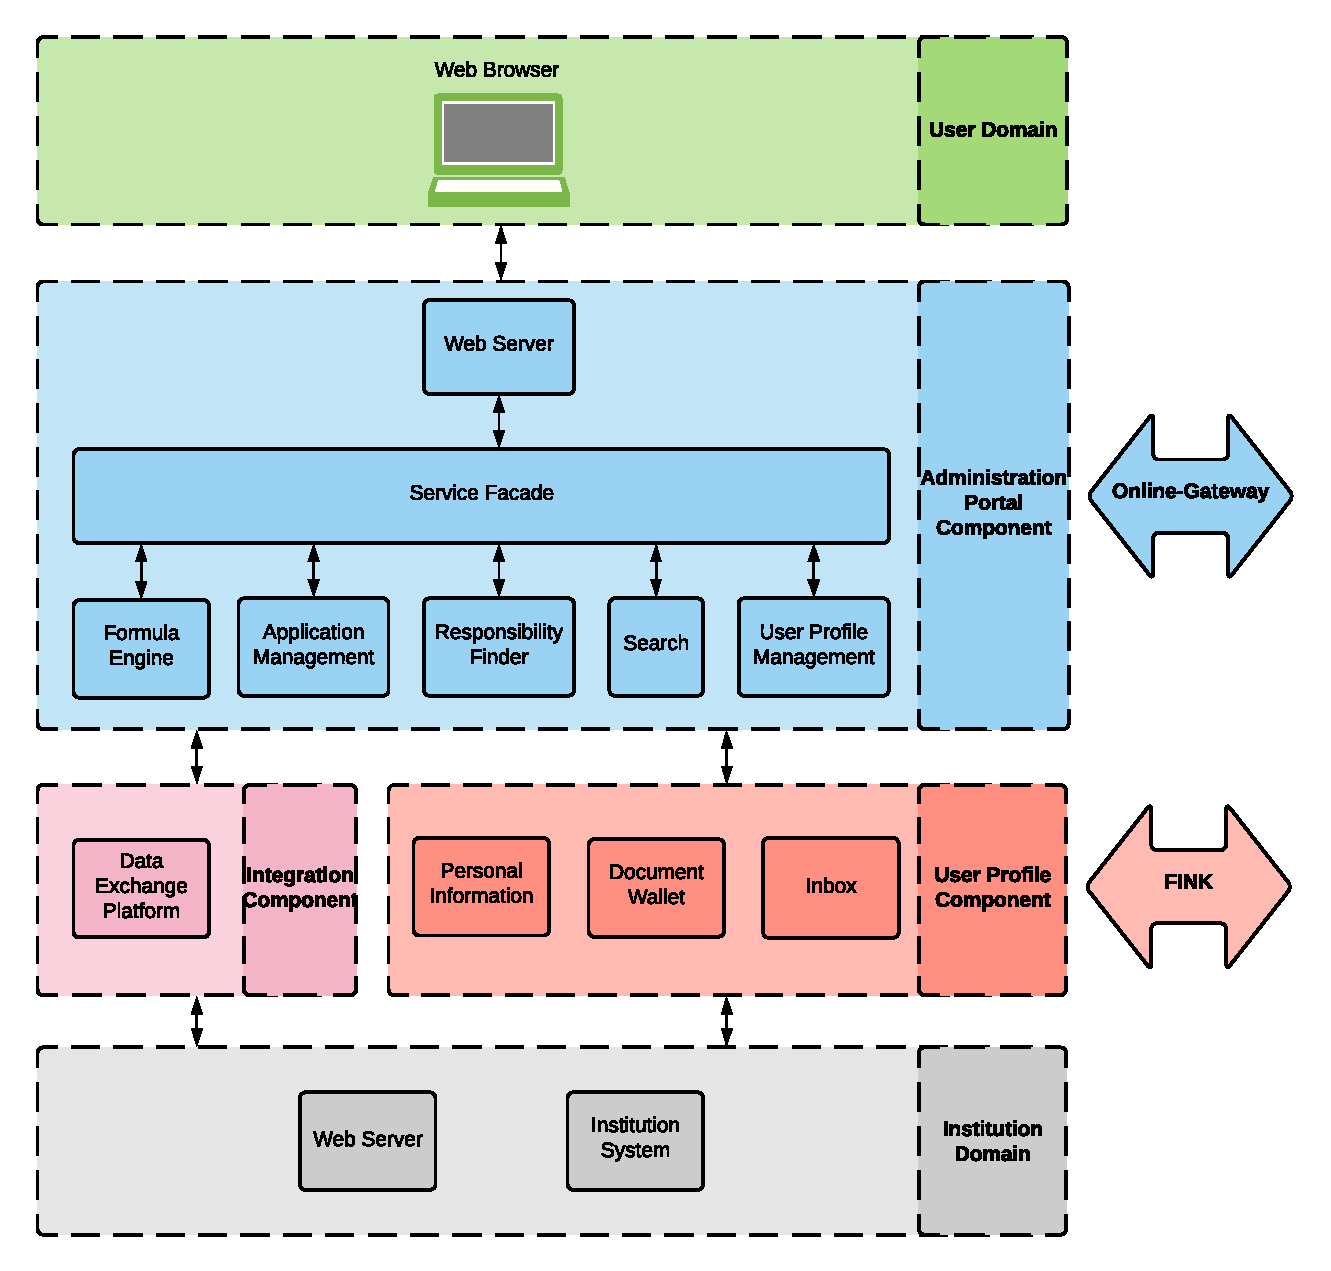
\includegraphics[scale=0.6]{Diagrams/OZG System Overview.pdf}
\end{center}

\paragraph{Administration Portal}
The administration portal is the component which directly interacts with users through a web site an provides the basic OZG use case through interaction with other system components. Through the web page of the portal, the user can create and manage his user profile, receive and send messages, upload and download documents, find administrative services, select an application form for an administrative service and be forwarded to the respective form server. Without direct visibility for the user, the portal also transmits personal information from the user profile to the form server, receives finished applications from the form server, determines responsible institutions and submits applications to the data exchange platform.
The administration portal consists of a web server, responsible for hosting web pages, and a facade for service components. The most important components, the service facade provides an interface for are:

\begin{itemize}
    \item \textbf{Responsibility Finder}
    
    This service component is used to find administrative institutions which are responsible for an application. Depending on the type of application and on the home address of the user, different institutions might be responsible.
    
    \item \textbf{Process Management}
    
    This service component manages when the administration portal has to start which process in order to provide the basic OZG use case described earlier.
    
    \item \textbf{Search}
    
    This service component creates a list of URLs of administrative services relevant for a specified search term. This enables the portal to provide a search functionality of administrative services for the user.
    
    \item \textbf{User Profile Management}
    
    This service component enables the administration portal to interact with the user profile component to retrieve JSON Web Tokens, update and read personal information and document wallet, to read messages of the inbox and sent messages to an institution.
    
    \item \textbf{Application Management}
    
    This service component manages applications issued through the administration portal through communication with the form server. The component enables the user to start an application by forwarding him to the correct form on the form server and optionally providing personal information to the form server. Form server and portal communicate about the status and content of the application. The user is able to keep track about the status of active applications through the profile, view their content, send messages to responsible institutions and cancel them.
    
\end{itemize}

\paragraph{Form-Server}
The from-server provides digital forms associated to administrative services. They can be accessed by a user profile through online self-service and submitted as applications to administrative institutions. The main services are \cite{dNRW:Standardisierungskonzeptzur}

\begin{itemize}
    \item \textbf{Retrieval of a digital form}
    
    There exist many administrative services and depending on the member state or commune, the required layout of the application can be different. Therefore, a system called federal information management (Föderales Informationsmanagement: FIM) is used to standardize administrative services. FIM consists of three categories of building blocks.
    
    \textit{Service blocks} contain human readable descriptions about a administrative service.
    
    \textit{Data field blocks} contain the standardized description of data fields required for the application of administrative services.
    
    \textit{Process blocks} contain standardized descriptions about the process of an administrative service.

    Relevant for the form-server are data field blocks. A data field block can contain one element of five categories.
    
    \textit{Data fields} are the "smallest entity" of a data field block and describes one standardized piece of information. Depending on the type of information - if it is for example a checkbox or input field - additional metadata is included.
    
    \textit{Data field groups} consist of multiple data fields and other data field groups, relating to a category of information. A data field group can for example be "person" or "company".
    
    \textit{Rules} describe all kinds of logical conditions of and between data fields. This includes for example the automatic validation of the correctness of an entered value or the activation and deactivation of data fields depending on an entered value.
    
    \textit{Code lists} are lists of predefined values the user can select. This can for example be a list of all countries.
    
    \textit{Data field schemata} is the combination of entities from all previously described categories and describes the structure of a form.
    
    The building blocks are centrally managed by federal republic, member states and communes. This simplifies the creation of for example a new form by reusing existing data schema blocks and adding additional required data fields to a new data field schema.
    
    Each data field block can be uniquely identified through an ID. Therefore, if the form-server is provided with a FIM-ID, he can retrieve the corresponding data filed block from the central storage.
    
    \item \textbf{Initiation of application}
    
    The from-server can be requested to initiate an application using a certain form based on a FIM ID of a data field schemata. Along with the request, an identification and authorisation of a user profile has to be passed. Additional personal information of the user profile can be passed for automated filling in of the form.
    
    \item \textbf{Status update}
    
    The form-server sends updates regarding the current status of the application.

    \item \textbf{Automatic filling in of form}
    
    If the form server was provided with personal information during the initiation request for an application, it can automatically fill in the form.
    
    \item \textbf{Presentation of form}
    
    The form server can host a website where it displays an interactive form. The user can access this website either through an URL or through a web component.
    
    \item \textbf{Application interruption}
    
    The application can be interrupted or aborted. Interruption may occur if the user stays inactive for a certain period of time while filling in the form. The user can also manually interrupt the editing process. If the application is interrupted, the form-server stores the unfinished application for a certain amount of time. The user can then access the application at a later time.
    
    If the user decides to cancel editing the form, the application is deleted from the from-server.
    
    Depending on the actions of the user, the status of the application changes accordingly and the form server sends an status update.
    
    \item \textbf{Storage of application}
    The form-server stores applications for a specified period of time if they were interrupted or submitted.
    
    \item \textbf{Provisioning stored applications}
    
    If the form server is provided an identification and authorisation of a user, it searches all stored applications which belong to the user and sends back a list of URLs, through which the user can access them.
    
    \item \textbf{Deletion of stored application}

    If the form server is provided an identification and authorisation of a user and an identification of an application, it can delete the stored application.

    \item \textbf{Manually filling in data fields}
    
    When the form is presented to the user, it can happen, that not all information could be automatically filled in. In this case, the form can be interactively filled in by the user.
    
    \item \textbf{Uploading documents}
    
    The user can add documents as attachments to an application. The documents can either be uploaded from the local machine or the data wallet of the user profile.

    \item \textbf{Submission of application}
    
    When the user submits the application by for example pressing a "submit" button, the form-server sends a status update. The finished application can now be transmitted to a requesting system.

\end{itemize}

\paragraph{User Profile}
Each member state provides its own user profile for identity management. The main services are \cite{NRW:Umsetzung}:

\begin{itemize}
    \item \textbf{Identification and Authentification} \cite{dNRW:Anbindungsleitfaden}
    
    The user profile can be used for identification by transmitting personal information like name and address after successfully authentification. Authentification is the verification of an authentication. Users can authenticate for the user profile for example through a username / password combination.
    
    \item \textbf{Determination Trust Level} \cite{dNRW:Anbindungsleitfaden}
    
    The trust level of a logged in user profile is determined while registration and usage. The user can register and login to the user profile using a username / password combination or the German ID card. The trust level "High" is only granted, if the user registered using the German ID card \textbf{AND} logs in using the German ID card. All other combinations of registration and login result in a "normal" trust level.
    
    \item \textbf{Management Personal Information} \cite{dNRW:Anbindungsleitfaden} 
    
    Personal information of the user profile can be modified. This requires the user to authenticate. In case the user profile is connected with an online identity card, some attributes like name and age can not be changed.
    
    \item \textbf{Provisioning Personal Information} \cite{dNRW:Anbindungsleitfaden} \cite{dNRW:Schnittstellen}

    The user profile can be requested to send personal information to a specified URL. This requires the user to authenticate.
    
\end{itemize}

\paragraph{Institution}
Institutions are the entities which eventually process the incoming applications and provide the users with solutions. They receive a digital application through the data-exchange platform and send back the result as a message through the inbox.

\paragraph{Data-Exchange Platform}
The data-exchange platform delivers applications from the administration portal to the correct administrative institution.

\paragraph{Data Wallet}
The data wallet is a sub-component of the user profile and enables the user to manage documents for his user profile. The main services are:

\begin{itemize}

    \item \textbf{Upload of document}
    
    The user can upload a document from his local machine to the data wallet.
    
    \item \textbf{Show documents}
    
    The user can list all documents which are stored in the data wallet.
    
    \item \textbf{Delete documents}
    
    The user can delete documents from the data wallet.
    
    \item \textbf{Attach documents to application}
    
    The user can attach a copy of a document stored in his data wallet to an application on a from server.

\end{itemize}

\paragraph{Inbox}
The inbox is a sub-component of the user profile and enables the user to send messages through his user profile. The main services are:
    
\begin{itemize}
    
    \item \textbf{Send a message}
    
    The user can send a message to authorities. This can be for example an institution which processes an application.
    
    \item \textbf{Receive a message}
    
    The user can receive messages from authorities for example to update the status of an application.
    
    \item \textbf{List messages}
    
    The user can see the messages he received by logging in to his user profile on the administration portal.
    
    \item \textbf{Notification through E-Mail}
    
    The user can be notified of a new message through E-Mail.

\end{itemize}

\subsubsection{Interfaces}
In order to implement the basic use case, the components have to interact with each. The following diagram visualizes, which components interact. Each interaction is described afterwards. The arrows describe the main direction of information flow in an interaction.

\begin{center}
    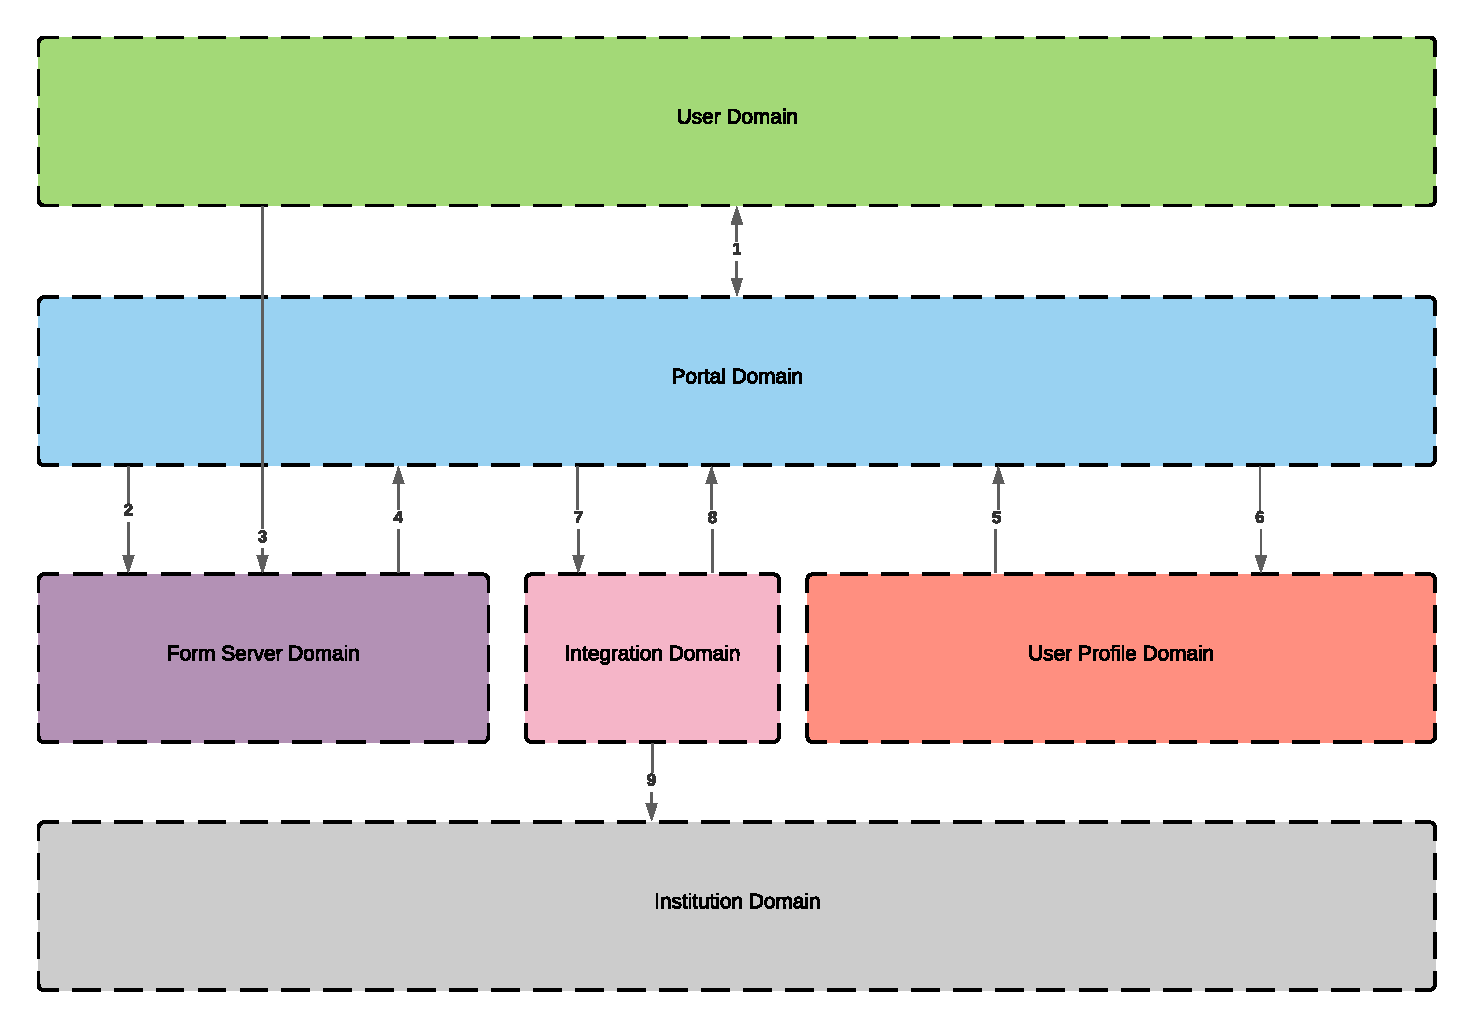
\includegraphics[scale=0.6]{Diagrams/Interaction Diagram.pdf}
\end{center}

\begin{enumerate}

    \item The web browser of the user displays the web pages hosted by the administration portal.

    \item The form-server can initiate the application if requested by the administration portal. The portal submits information for identification, authentication and authorisation of a user through an JSON Web Token and a user profile ID. In order for the form server to determine the correct form to display, the portal submits a FIM-ID which corresponds to a data field schemata. In case the user approved, the portal can also collect personal information from the user profile and submit it to the form server for automated filling in of the form.
    
    \item The form server provides the user a web page which displays an interactive form.
    
    \item The form server notifies the administration portal of changes in the status of applications. If the administration portal is notified of a submitted application, it requests the form server to transmit the application data.
    
    \item The administration portal requests the user profile for identification and authentication to login a user on the web page of the portal. The portal also requests authorisation from the user profile to for example access certain personal information.
    
    \item The administration portal enables the user to manage services of the user profile. It provides OSS tools for managing attributes stored in the user profile, to send new messages and to manage documents in the data wallet.
    
    \item The administration platform submits application data to the data exchange platform for delivery to the responsible institution.
    
    \item The data exchange platform notifies the administration portal of the delivery status of the application data.
    
    \item The data exchange platform notifies the institution of a new application and enables it to download the corresponding data.
    
    \item The institution can send messages to the inbox of a user profile to for example request additional documents.
    
    \item The user can send messages to the institution which for example asked for additional documents.
    
\end{enumerate}
    
\subsubsection{Data Objects}
This section describes what data each component processes. The property value describes a certain type of data. The source describes which component stores the value. This distinguishes the access of a property by reference and by copy. If the source of a property is another component, the property is accessed by reference. The description gives further detail on how the property is processed by the component.

\begin{table}[!h]
    \begin{tabularx}{\textwidth}{|l|l|l|C|}
    \rowcolor{LightCyan}
    \hline
    \multicolumn{4}{|l|}{Administration Portal: Service Web Page} \\
    \hline
    Property & Storage & Origin & Description  \\
    \hline
    \hline
    Name & Web Page & FIM & Name of an administrative service \\
    \hline
    URL & Portal & Portal & The URL of the Web Page \\
    \hline
    Description & Web Page & FIM & Description of an administrative service \\
    \hline
    FIM-ID & Web Page & FIM & FIM-ID of a data field schemata which describes attributes required from the user when applying for the service \\
    \hline
    \end{tabularx}
\end{table}

\begin{table}[!h]
    \begin{tabularx}{\textwidth}{|l|l|l|C|}
    \rowcolor{LightCyan}
    \hline
    \multicolumn{4}{|l|}{Administration Portal: User} \\
    \hline
    Property & Storage & Origin & Description  \\
    \hline
    \hline
    Attributes & User Profile & User Profile & The portal can manage attributes of user profiles \\
    \hline
    JWT & Portal & User Profile & The portal can retrieve a JSON Web Token from the profile after successful authentication by a user \\
    \hline
    URL Form & Portal & Form Server & The portal stores the URL where the form server hosts the interactive form \\
    \hline
    \end{tabularx}
\end{table}

\begin{table}[!h]
    \begin{tabularx}{\textwidth}{|l|l|l|C|}
    \rowcolor{LightCyan}
    \hline
    \multicolumn{4}{|l|}{Administration Portal: Application} \\
    \hline
    Property & Storage & Origin & Description  \\
    \hline
    \hline
    FMS-ID & Portal & Form Server & The portal receives the ID of applications from the form server \\
    \hline
    Status & Portal & Form Server & The portal receives status updates for each application \\
    \hline
    XML Form Data & Portal & Form Server & The portal can retrieve the data which was filled into a form \\
    \hline
    \end{tabularx}
\end{table}

\begin{table}[!h]
    \begin{tabularx}{\textwidth}{|l|l|l|C|}
    \rowcolor{LightCyan}
    \hline
    \multicolumn{4}{|l|}{User Profile: Personal Information} \\
    \hline
    Property & Storage & Origin & Description  \\
    \hline
    \hline
    Attributes & User Profile & FIM & The list of attributes the user can fill in at his profile are based on FIM data fields managed in the FIM repository. \\
    \hline
    Attribute Values & User Profile & User & The user can manually add values to a list of predetermined attributes in his profile \\
    \hline
    Credentials & User Profile & User & The User Profile stores encrypted credentials of the user to authenticate him \\
    \hline
    User Profile ID & User Profile & User Profile & The User Profile creates and stores a unique ID for the user \\
    \hline
    \end{tabularx}
\end{table}

\begin{table}[!h]
    \begin{tabularx}{\textwidth}{|l|l|l|C|}
    \rowcolor{LightCyan}
    \hline
    \multicolumn{4}{|l|}{User Profile: Authorisatiozation} \\
    \hline
    Property & Storage & Origin & Description  \\
    \hline
    \hline
    JWT & Other Component & User Profile & The user profile can create and transfer JSON Web Tokens which authorise other components to access resources of the user profile \\
    \hline
    \end{tabularx}
\end{table}

\begin{table}[!h]
    \begin{tabularx}{\textwidth}{|l|l|l|C|}
    \rowcolor{LightCyan}
    \hline
    \multicolumn{4}{|l|}{User Profile: Inbox} \\
    \hline
    Property & Storage & Origin & Description  \\
    \hline
    \hline
    Received Messages & User Profile & User & The user profile stores messages which were addressed to the user \\
    \hline
    Sent Messages & User Profile & User & The user profile stores messages which were sent by the user \\
    \hline
    \end{tabularx}
\end{table}

\begin{table}[!h]
    \begin{tabularx}{\textwidth}{|l|l|l|C|}
    \rowcolor{LightCyan}
    \hline
    \multicolumn{4}{|l|}{User Profile: Data Wallet} \\
    \hline
    Property & Storage & Origin & Description  \\
    \hline
    \hline
    Documents & User Profile & User & The user profile stores documents which were uploaded by the user \\
    \hline
    \end{tabularx}
\end{table}

\begin{table}[!h]
    \begin{tabularx}{\textwidth}{|l|l|l|C|}
    \rowcolor{LightCyan}
    \hline
    \multicolumn{4}{|l|}{Form Server} \\
    \hline
    Property & Storage & Origin & Description  \\
    \hline
    \hline
    FMS-ID & Form Server & Form Server & The form server creates a unique ID for each application \\
    \hline
    JWT & Form Server & User Profile & The form server uses a JSON Web Token to verify that the entity issuing the request is authorised \\
    \hline
    User Profile ID & Form Server & User Profile & The ID of the user who is associated to the application \\
    \hline
    FIM-ID & Form Server & FIM & The FIM ID of a data field schemata is used to determine how to construct the form \\
    \hline
    Form & Form Server & FIM & The list of attributes the user can fill in at the form are based on the FIM data field schemata. The form server maps the FIM data fields of the FIM data field schemata to attributes the form server understands \\
    \hline
    Status & Form Server & Form Server & The status describes which actions were performed on the application \\
    \hline
    Application Data & Form Server & User & The form server stores the data which the user filled in to the form as an XML file \\
    \hline
    Web Page & Form Server & Form Server & The form server hosts a web page with the interactive form  \\
    \hline 
    Web Page URL & Form Server & Form Server & The form server hosts the web page of the form at an individual URL \\
    \hline 
    \end{tabularx}
\end{table}

\subsubsection{Sequence Diagram}

\begin{figure}[!h]
    \centering
    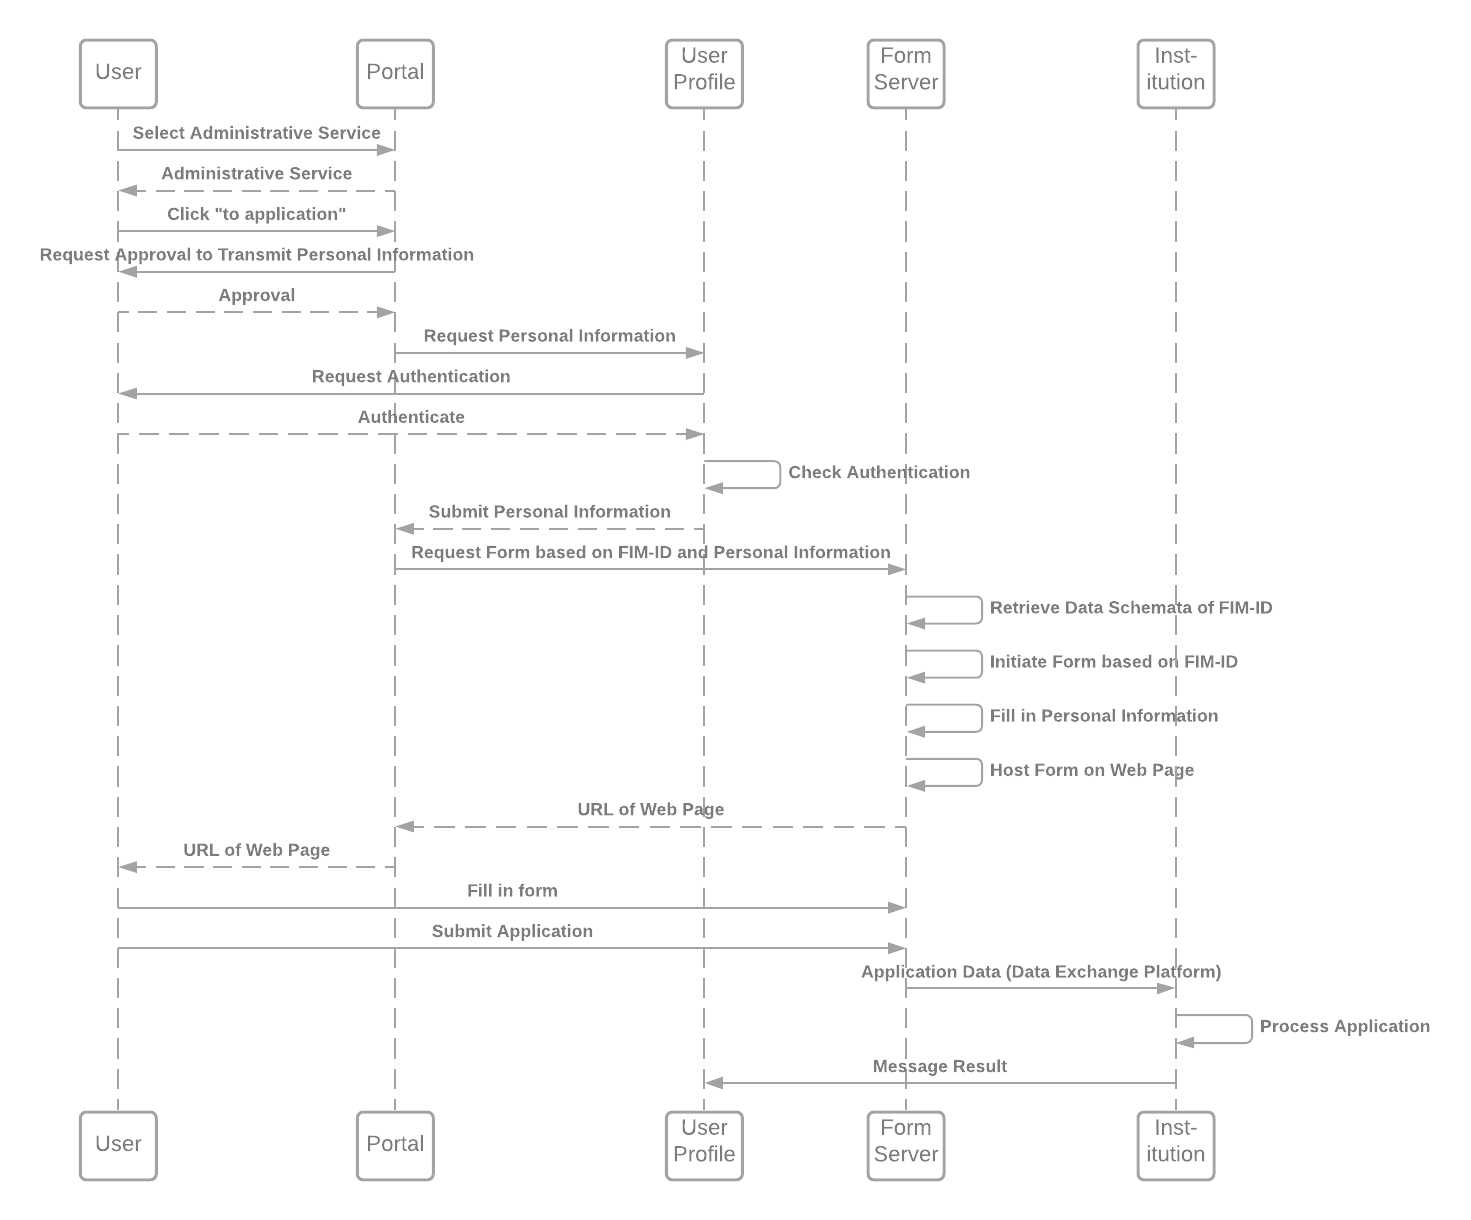
\includegraphics[width=17cm]{Diagrams/Basic Use Case Sequence Diagram.png}
\end{figure}
